\documentclass[10pt]{article}
\usepackage[letterpaper]{geometry}
\geometry{verbose,tmargin=1in,bmargin=1in,lmargin=1in,rmargin=1in}
\usepackage{setspace}
\usepackage{ragged2e}
\usepackage{color}
\usepackage{titlesec}
\usepackage{graphicx}
\usepackage{float}
\usepackage{mathtools}
\usepackage{amsmath}
\usepackage[font=small,labelfont=bf,labelsep=period]{caption}
\usepackage[english]{babel}
\usepackage{indentfirst}
\usepackage{array}
\usepackage{makecell}
\usepackage[usenames,dvipsnames]{xcolor}
\usepackage{multirow}
\usepackage{tabularx}
\usepackage{arydshln}
\usepackage{caption}
\usepackage{subcaption}
\usepackage{xfrac}
\usepackage{etoolbox}
\usepackage{cite}
\usepackage{url}
\usepackage{dcolumn}
\usepackage{hyperref}
\usepackage{courier}
\usepackage{url}
\usepackage{esvect}
\usepackage{commath}
\usepackage{verbatim} % for block comments
\usepackage{enumitem}
\usepackage{hyperref} % for clickable table of contents
\usepackage{braket}
\usepackage{titlesec}
\usepackage{booktabs}
\usepackage{gensymb}
\usepackage{longtable}
\usepackage{soul} % for striking out text
\usepackage[makeroom]{cancel}	% to cancel out text

\usepackage{listings}
\lstset{
    frame=single,
    breaklines=true,
    postbreak=\raisebox{0ex}[0ex][0ex]{\ensuremath{\color{red}\hookrightarrow\space}}
}

% for circled numbers
\usepackage{tikz}
\newcommand*\circled[1]{\tikz[baseline=(char.base)]{
            \node[shape=circle,draw,inner sep=2pt] (char) {#1};}}


\titleclass{\subsubsubsection}{straight}[\subsection]

% define new command for triple sub sections
\newcounter{subsubsubsection}[subsubsection]
\renewcommand\thesubsubsubsection{\thesubsubsection.\arabic{subsubsubsection}}
\renewcommand\theparagraph{\thesubsubsubsection.\arabic{paragraph}} % optional; useful if paragraphs are to be numbered

\titleformat{\subsubsubsection}
  {\normalfont\normalsize\bfseries}{\thesubsubsubsection}{1em}{}
\titlespacing*{\subsubsubsection}
{0pt}{3.25ex plus 1ex minus .2ex}{1.5ex plus .2ex}

\makeatletter
\renewcommand\paragraph{\@startsection{paragraph}{5}{\z@}%
  {3.25ex \@plus1ex \@minus.2ex}%
  {-1em}%
  {\normalfont\normalsize\bfseries}}
\renewcommand\subparagraph{\@startsection{subparagraph}{6}{\parindent}%
  {3.25ex \@plus1ex \@minus .2ex}%
  {-1em}%
  {\normalfont\normalsize\bfseries}}
\def\toclevel@subsubsubsection{4}
\def\toclevel@paragraph{5}
\def\toclevel@paragraph{6}
\def\l@subsubsubsection{\@dottedtocline{4}{7em}{4em}}
\def\l@paragraph{\@dottedtocline{5}{10em}{5em}}
\def\l@subparagraph{\@dottedtocline{6}{14em}{6em}}
\makeatother

\newcommand{\volume}{\mathop{\ooalign{\hfil$V$\hfil\cr\kern0.08em--\hfil\cr}}\nolimits}

\setcounter{secnumdepth}{4}
\setcounter{tocdepth}{4}
\begin{document}

\textbf{NE 255: HW4}3\hfill April Novak\newline

\circled{1} The \(S_N\) equations provide the framework to discretize the angular flux in angle, but the equations still must be discretized in space. In general, there are two different means to perform spatial discretization - cell balance methods, which preserve conservation of the solution, and finite element methods, which do not necessarily preserve conservation of the solution. In a single mesh cell, cell balance methods will provide a statement that is equivalent to conservation of neutrons, while finite element methods satisfy the governing equation in a weighted-integral sense. For simplicity, all of the spatial discretization schemes discussed here are applied to the simplified transport equation that neglects time dependence and assumes some angular discretization has already been applied to \(\psi\) such that it is independent of angle (in each of these equations):

\begin{equation}
\label{eq:SimpleTE}
\hat{\Omega}\cdot\nabla\psi(\vv{r},E)+\Sigma_t({\vv{r},E})\psi(\vv{r},E)=S(\vv{r},E)
\end{equation}

where \(S\) represents the scattering, fission, and external sources. There will be one of these equations for each discrete direction in the \(S_N\) method. For all the following discretization schemes, a Cartesian mesh given in the figure in the \texttt{spatial-disr.pdf} is assumed, with \(i\) representing indices in the \(x\)-direction, \(j\) in the \(y\)-direction, and \(k\) in the \(z\)-direction.

Cell balance schemes point values for the solution \(\psi\) over a discretized spatial mesh. With the definitions for the components of \(\hat{\Omega}\) as \(\hat{\Omega}=\mu\hat{x}+\eta\hat{y}+\xi\hat{z}\), integrating Eq. \eqref{eq:SimpleTE} over the mesh cell gives:

\begin{equation}
\int_{x_{i-1/2}}^{x_{i+1/2}}dx\mu \frac{\partial \psi}{\partial x}+\int_{y_{j-1/2}}^{y_{j+1/2}}dy\eta \frac{\partial \psi}{\partial y}+\int_{z_{k-1/2}}^{z_{k+1/2}}dz\xi \frac{\partial \psi}{\partial z}+\Sigma_{t,ijk}{E}\psi_{ijk}(\vv{r},E)=S_{ijk}(E)
\end{equation}

where it has been assumed that \(\Sigma_t\) and \(S\) are constant over the cell, and are represented by their cell-centered values. In addition, the energy-dependence has been dropped. Without approximation, the integrals in the above reduce to:

\begin{equation}
\label{eq:DiscretizedCartesianTE}
\frac{\mu}{\Delta_i}(\psi_{i+1/2}-\psi_{i-1/2})+\frac{\eta}{\Delta_j}(\psi_{j+1/2}-\psi_{j-1/2})+\frac{\xi}{\Delta_k}(\psi_{k+1/2}-\psi_{k-1/2})+\Sigma_{t,ijk}\psi_{ijk}=S_{ijk}
\end{equation}

With this discretization method, there must be some way to relate the cell-centered value \(ijk\) to the face values. The different options we have for discretization are related to the choices we can make for how to relate these quantities. The Diamond Difference and Step Difference schemes choose the following relationship:

\begin{equation}
\label{eq:DifferencingRelationship}
\psi_{i\pm1/2}=\frac{2}{1\pm\alpha}\psi_{ijk}-\frac{1\mp\alpha}{1\pm\alpha}\bar{\psi}_{i\mp1/2}
\end{equation}

and likewise for the \(y\) and \(z\) directions. \(\bar{\psi}\) represents a known flux, and depending on whether a sweep is being performed in the positive-\(\mu\) direction (\(\bar{\psi}_{i-1/2}\) is known) or in the negative-\(\mu\) direction (\(\bar{\psi}_{i+1/2}\) is known), either the + or - option is selected in Eq. \eqref{eq:DifferencingRelationship}. Once the sweep direction is known, the relationship in Eq. \eqref{eq:DifferencingRelationship} is used in the governing equation Eq. \eqref{eq:DiscretizedCartesianTE} to solve for the cell-centered flux in terms of only known quantities:

\begin{equation}
\label{eq:psi_ijk}
\psi_{ijk}=\frac{S_{ijk}+\frac{2}{1\pm\alpha}\left(\frac{|\mu|}{\Delta_i}\bar{\psi}_{i\mp1/2}+\frac{|\eta|}{\Delta_j}\bar{\psi}_{j\mp1/2}+\frac{|\xi|}{\Delta_k}\bar{\psi}_{k\mp1/2}\right)}{\Sigma_{t,ijk}+\frac{2}{1\pm\alpha}\left(\frac{|\mu|}{\Delta_i}+\frac{|\eta|}{\Delta_j}+\frac{|\xi|}{\Delta_k}\right)}
\end{equation}

where it has been assumed that \(\alpha\) is selected to be the same in all directions. \(\alpha\) is a parameter used to tune the spatial discretization. Common choices for \(\alpha\) have their own names. The Diamond Difference method sets \(\alpha=0\). With this choice, the cell-centered flux is an average of the face fluxes. The Step Difference method, on the other hand, sets \(\alpha=\pm1\) such that the cell-centered flux is set equal to the incoming face flux (choose 1 or -1 accordingly so that Eq. \eqref{eq:DifferencingRelationship} provides an expression for \(\psi_{ijk}\) in terms of the known incoming face flux).The Diamond Difference method is second-order in space, while the Step Difference method is only first-order. 

The objective is to choose the correct relationship in Eq. \eqref{eq:DifferencingRelationship} such that the known quantities, or the incoming fluxes to each cell, can be used to compute the unknown quantities, or the outgoing fluxes for each cell, in a ``sweep'' over the spatial mesh. Each of these sweeps is performed for each individual flux \(\psi(\hat{\Omega}_a\). Now that the numerical method has been set up, the sweeping process can be described in more detail for the different situations prompted in the homework:\newline

\textbf{(a)}: For a sweep in the positive-\(\mu\) direction, we supposedly know \(\bar{\psi}_{i-1/2}\), so we would relate the cell-centered flux to the outgoing flux in the following way:

\begin{equation}
\label{eq:PositiveMu}
\begin{aligned}
\psi_{i+1/2}=\frac{2}{1+\alpha}\psi_{ijk}-\frac{1-\alpha}{1+\alpha}\bar{\psi}_{i-1/2}\quad\rightarrow\quad\psi_{ijk}=\frac{1}{2}\left\lbrack(1+\alpha)\psi_{i+1/2}+(1-\alpha)\bar{\psi}_{i-1/2}\right\rbrack\\
\end{aligned}
\end{equation}

So, to perform the sweep, we would begin at the boundary at which a boundary condition is specified. At this boundary, the incoming flux \(\bar{\psi}_{i-1/2}\) is known. Then, Eq. \eqref{eq:psi_ijk} is used to determine the cell-centered flux \(\psi_{ijk}\). Then, finally, Eq. \eqref{eq:PositiveMu} is used to compute the outgoing fluxes from the cell-centered fluxes. To be more precise, the steps for a Diamond Difference method (\(\alpha=0\)) are:

\begin{enumerate}
\item Begin at the boundary at which the incoming fluxes are known. Compute the cell-centered fluxes using:

\begin{equation}
\psi_{ijk}=\frac{S_{ijk}+2\left(\frac{|\mu|}{\Delta_i}\bar{\psi}_{i-1/2}+\frac{|\eta|}{\Delta_j}\bar{\psi}_{j-1/2}+\frac{|\xi|}{\Delta_k}\bar{\psi}_{k-1/2}\right)}{\Sigma_{t,ijk}+2\left(\frac{|\mu|}{\Delta_i}+\frac{|\eta|}{\Delta_j}+\frac{|\xi|}{\Delta_k}\right)}
\end{equation}

\item Then, compute the outgoing fluxes using:

\begin{equation}
\psi_{i+1/2}=2\psi_{ijk}-\bar{\psi}_{i-1/2}
\end{equation}

\item Repeat steps 1 and 2 for the remaining cells, using the outgoing fluxes from step 2 as the new incoming fluxes in step 1. If there is no fission, scattering, or external source, then only one sweep is needed. On the other hand, if any of these sources are present, then after each sweep, an updated source \(S_{ijk}\) must be computed, and the process repeated until reaching convergence.
\end{enumerate}

\textbf{(b)}: For a sweep in the negative-\(\mu\) direction, we supposedly know \(\bar{\psi}_{i+1/2}\), so we would relate the cell-centered flux to the outgoing flux in the following way:

\begin{equation}
\label{eq:NegativeMu}
\begin{aligned}
\psi_{i-1/2}=\frac{2}{1-\alpha}\psi_{ijk}-\frac{1+\alpha}{1-\alpha}\bar{\psi}_{i+1/2}\quad\rightarrow\quad\psi_{ijk}=\frac{1}{2}\left\lbrack(1+\alpha)\psi_{i+1/2}+(1-\alpha)\bar{\psi}_{i-1/2}\right\rbrack\\
\end{aligned}
\end{equation}

Very similar to a sweep in the positive direction, we would begin at the boundary at which a boundary condition is specified. At this boundary, the incoming flux \(\bar{\psi}_{i+1/2}\) is known. Then, Eq. \eqref{eq:psi_ijk} is used to determine the cell-centered flux \(\psi_{ijk}\). Then, finally, Eq. \eqref{eq:NegativeMu} is used to compute the outgoing fluxes from the cell-centered fluxes. To be more precise, the steps for a Diamond Difference method (\(\alpha=0\)) are:

\begin{enumerate}
\item Begin at the boundary at which the incoming fluxes are known. Compute the cell-centered fluxes using:

\begin{equation}
\psi_{ijk}=\frac{S_{ijk}+2\left(\frac{|\mu|}{\Delta_i}\bar{\psi}_{i+1/2}+\frac{|\eta|}{\Delta_j}\bar{\psi}_{j+1/2}+\frac{|\xi|}{\Delta_k}\bar{\psi}_{k+1/2}\right)}{\Sigma_{t,ijk}+2\left(\frac{|\mu|}{\Delta_i}+\frac{|\eta|}{\Delta_j}+\frac{|\xi|}{\Delta_k}\right)}
\end{equation}

\item Then, compute the outgoing fluxes using:

\begin{equation}
\psi_{i-1/2}=2\psi_{ijk}-\bar{\psi}_{i+1/2}
\end{equation}

\item Repeat steps 1 and 2 for the remaining cells, using the outgoing fluxes from step 2 as the new incoming fluxes in step 1. If there is no fission, scattering, or external source, then only one sweep is needed. On the other hand, if any of these sources are present, then after each sweep, an updated source \(S_{ijk}\) must be computed, and the process repeated until reaching convergence.
\end{enumerate}

The only difference between a sweep in the positive and negative \(\mu\)-directions is the notation on which flux is known - either \(\psi_{i+1/2}\) or \(\psi_{i-1/2}\) is known.\newline

\textbf{(c)} If reflective boundary conditions are present, then begin from the side of the domain for which the conditions are known. Apply steps 1-3 listed in part (a) (if moving in the \(\mu>0\) direction) or steps 1-3 listed in part (b) (if moving in the \(\mu<0\) direction) in order to reach the reflecting boundary from a boundary at which the incoming flux is known. Using the equations in either (a) or (b) is determined by which boundary has values specified - begin from that boundary, and sweep until reaching the reflecting boundary. Then, once at the reflecting boundary, apply the condition that \(\psi_{N+1, i+1/2}=\psi_{N+1, i-1/2}\), where \(N\) is the number of mesh cells such that \(N+1\) is the number of the node on the right face, assuming a linear, Cartesian grid. This condition is applied such that a sweep then begins moving in the opposite direction of the first sweep (and so apply steps 1-3 in part (a) if initially the steps from part (b) were applied, and vice versa. These steps are not repeated here to avoid redundancy). After each double sweep, updates are performed to \(S_{ijk}\). This process is repeated until reaching convergence. If reflective boundary conditions exist on both ends of the domain, then an initial guess for the incoming fluxes at the starting point must be made, and then each double sweep is again halted to perform updates to \(S_{ijk}\) until reaching convergence.\newline

\textbf{(d)} In a single sweep, each cell requires that the incoming fluxes and source \(S_{ijk}\) to proceed with the sweep. To compute \(S_{ijk}\), the scattering, fission, and external source, we need to have all flux moments for that cell. Once an updated \(S_{ijk}\) is computed however, those flux moments can be discarded, except those that contribute to the incoming flux of the next cell. So, as we sweep through the mesh, once a cell computation is complete, the incoming and cell-centered flux values for that cell can be discarded so long as \(S_{ijk}\) has been updated for the next sweep.\newline

\circled{2} Truncation error can be quantified for a 1-D, zero-source flux. This flux signifies the flux of neutrons moving with angle \(\hat{\Omega}_a\), but for simplicity the \(a\) subscripts on \(\psi\) and \(\mu\) are not retained throughout this problem, but are left to be implied.\newline

\textbf{(a)}: The equation to be solved analytically is:

\begin{equation}
\label{eq:Ex2}
\mu\frac{d\psi}{dx}+\Sigma_t\psi=0
\end{equation}

The analytical solution to this equation is:

\begin{equation}
\frac{d\psi}{\psi}=\frac{-\Sigma_t}{|\mu|}dx\quad\rightarrow\quad\int_{x}^{x^{'}}\frac{d\psi}{\psi}=\int_{x}^{x^{'}}\frac{-\Sigma_t}{|\mu|}dx
\end{equation}

Performing the integration:

\begin{equation}
\label{eq:124}
\ln{\left(\frac{\psi_{x^{'}}}{\psi_{x}}\right)}=\frac{-\Sigma_t}{|\mu|}\delta_i\quad\rightarrow\quad\psi_{x^{'}}=\exp{\left(\frac{-\Sigma_t}{|\mu|}\delta_i\right)}\psi_{x}
\end{equation}

where \(\delta_i\equiv x^{'}-x\).\newline

\textbf{(b)}: For a Cartesian grid with \(x^{'}=x_{i+1/2}\) and \(x=x_{i-1/2}\), Eq. \eqref{eq:124} becomes:

\begin{equation}
\label{eq:128}
\psi_{i+1/2}=\exp{\left(\frac{-\Sigma_t}{|\mu|}\Delta_i\right)}\psi_{i-1/2}
\end{equation}

\begin{equation}
\label{eq:1241}
\ln{\left(\frac{\psi_{i+1/2}}{\psi_{i-1/2}}\right)}=\frac{-\Sigma_t}{|\mu|}\Delta_i\quad\rightarrow\quad\psi_{i+1/2}=\exp{\left(\frac{-\Sigma_t}{|\mu|}\delta_i\right)}\psi_{i-1/2}
\end{equation}

where \(\Delta_i\equiv x_{i+1/2}-x_{i-1/2}\). Introducing the definition \(h=\Sigma_t\Delta_i/2|\mu|\), the above becomes:

\begin{equation}
\label{eq:128}
\ln{\left(\frac{\psi_{i+1/2}}{\psi_{i-1/2}}\right)}=-2h\quad\rightarrow\quad\psi_{i+1/2}=\exp{\left(-2h\right)}\psi_{i-1/2}
\end{equation}

\textbf{(c)}: To determine the numerical equivalent of Eq. \eqref{eq:128}, the diamond difference equations give \(\psi_{ijk}\) in terms of the face flux values as:

\begin{equation}
\label{eq:2c}
\psi_{i+1/2}=2\psi_{ijk}-\bar{\psi}_{i-1/2}
\end{equation}

The discretized form of the transport equation is already given in Eq. \eqref{eq:DiscretizedCartesianTE}. Inserting Eq. \eqref{eq:2c} into the 1-D form of Eq. \eqref{eq:DiscretizedCartesianTE} (with the source term neglected for this specific problem) for \(\psi_{ijk}\) gives a second relationship between \(\psi_{i+1/2}\) and \(\psi_{i-1/2}\):

\begin{equation}
\frac{\mu}{\Delta_i}(\psi_{i+1/2}-\psi_{i-1/2})+\Sigma_{t}\frac{1}{2}\left(\psi_{i+1/2}+\psi_{i-1/2}\right)=0
\end{equation}

Rearranging, and inserting the definition for \(h\):

\begin{equation}
\label{eq:PositiveConditon}
\psi_{i+1/2}=\frac{1-h}{1+h}\psi_{i-1/2}
\end{equation}

\textbf{(d)}: The power series of \(e^{-2h}\) is:

\begin{equation}
\label{eq:23}
e^{-2h}\approx1+(-2h)+\frac{(-2h)^2}{2!}+\cdots=1-2h-2h^2+\cdots
\end{equation}

The coefficient in Eq. \eqref{eq:PositiveConditon} can be written as:

\begin{equation}
\frac{1-h}{1+h}=\frac{(1-h)^2}{1-h^2}=(1-h)^2\sum_{i=0}^\infty(h^2)^n\approx(1-h)^2\left(1+(h^2)+\frac{h^4}{2}+\cdots\right)
\end{equation}

Expanding the first term in the above equation fully:

\begin{equation}
\label{eq:22}
\frac{1-h}{1+h}\approx(1-h)^2+\cdots=1-2h-h^2+\cdots
\end{equation}

By comparing Eq. \eqref{eq:22} with Eq. \eqref{eq:23}, it can be seen that the truncation error is very nearly second order, and hence the discretization is of second order. 

\textbf{(e)}: From Eq. \eqref{eq:PositiveConditon}, it is clear that \(\psi_{i+1/2}\) could be negative if \(h>1\). In other words, from the definition of \(h\), the flux can be negative if:

\begin{equation}
\label{eq:NegativeCondition}
\Delta_i>\frac{2|\mu|}{\Sigma_t}
\end{equation}

From a cost perspective, the coarser the mesh, the better, since then the simulation will not be overly-limited by the mesh requirements. The conditions for which the mesh refinement will cause the most complications (i.e. produce negative fluxes) is for small \(|\mu|\) or large \(\Sigma_t\). In order to avoid negative fluxes, we require \(\Delta_i<\frac{2|\mu|}{\Sigma_t}\).\newline 

\circled{3} For this problem, the boundary conditions are:

\begin{equation}
\begin{aligned}
\psi(0)=0 \text{ for } \mu>0\\
\psi(2) \text{ for } \mu>0 = \psi(2) \text{ for } \mu<0\\
\end{aligned}
\end{equation}

Due to the reflecting boundary conditions present at \(x=2\), sweeps in both the positive and negative \(\mu\) directions are needed. The numerical algorithm is:

\begin{enumerate}
\item Begin at \(x=0\) with the boundary condition \(\psi_{i-1/2}=0\). 
\item Compute the cell-centered flux using:

\begin{equation}
\psi_{i}=\frac{S_{i}+\frac{2}{1+\alpha}\left(\frac{|\mu|}{\Delta_i}\bar{\psi}_{i-1/2}\right)}{\Sigma_{t,i}+\frac{2}{1+\alpha}\left(\frac{|\mu|}{\Delta_i}\right)}
\end{equation}

\item Compute the outgoing face flux using:

\begin{equation}
\psi_{i+1/2}=\frac{2}{1+\alpha}\psi_{ijk}-\frac{1-\alpha}{1+\alpha}\bar{\psi}_{i-1/2}
\end{equation}

\item Repeat steps 2 and 3 until reaching the very last cell. At the last cell, after performing step 3, the outgoing flux has been computed. This must be reflected to serve as the incoming flux for a sweep in the negative-\(\mu\) direction. At the last cell, set \(\psi_{i+1/2}=\psi_{i+1/2}\) to serve as the incoming face flux for a sweep in the negative-\(\mu\) direction.

\item Begin the sweep in the negative-\(\mu\) direction. Compute the cell-centered flux using:

\begin{equation}
\psi_{i}=\frac{S_{i}+\frac{2}{1-\alpha}\left(\frac{|\mu|}{\Delta_i}\bar{\psi}_{i+1/2}\right)}{\Sigma_{t,i}+\frac{2}{1-\alpha}\left(\frac{|\mu|}{\Delta_i}\right)}
\end{equation}

\item Compute the outgoing face flux using:

\begin{equation}
\psi_{i-1/2}=\frac{2}{1-\alpha}\psi_{ijk}-\frac{1+\alpha}{1-\alpha}\bar{\psi}_{i+1/2}
\end{equation}

\item Repeat steps 5 and 6 for all cells until reaching the very first cell again. At this point, if there is no source (fission, scattering, or external), then no further sweeps are needed, and the solution is complete.
\end{enumerate}

\textbf{(a)}: Using the numerical algorithm described above, Fig. \ref{fig:1} shows the angular flux for positive \(\mu\) and negative \(\mu\) (no quadrature rule has been applied to obtain the scalar flux yet), for a mesh spacing of \(h=0.08\). This is included purely to show some results before the quadrature is applied. 

\begin{figure}[H]
  \centering
  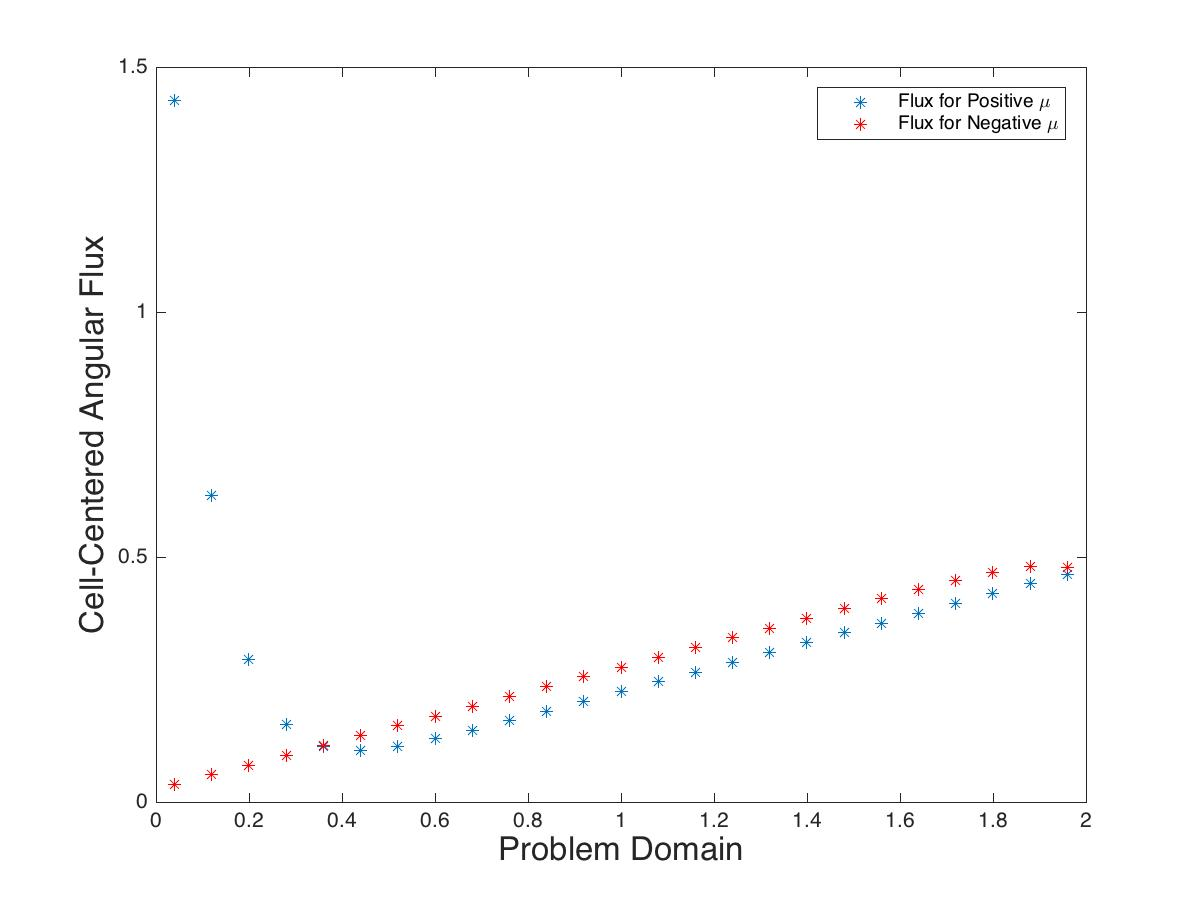
\includegraphics[width=12cm]{AngularFluxh08.jpg} % versioned
  \caption{Angular flux for positive and negative \(\mu\) for \(h=0.08\).}
  \label{fig:1}
\end{figure}

To obtain the scalar flux, the angular flux must be integrated over angle:

\begin{equation}
\phi=\int_{-1}^{1}\psi(\mu)d\mu\approx\sum_{i=1}^{N}w_i\psi(\mu_i)
\end{equation}

This integration is approximated with a quadrature rule. Because there is only one value of \(|\mu|\), \(\mu_i=0.1\), and because the problem statement says to use equi-probable weights, the weights are set to \(w_i=1.0\) so that integration over \(-1\leq\mu\leq1\) gives 2 if the angular flux is not dependent on angle. Note that this is not a real quadrature set. With this quadrature rule, Fig. \ref{fig:20} shows the scalar flux for \(h=0.08, 0.1, 0.125, 0.2, 0.4\). 

\begin{figure}[H]
  \centering
  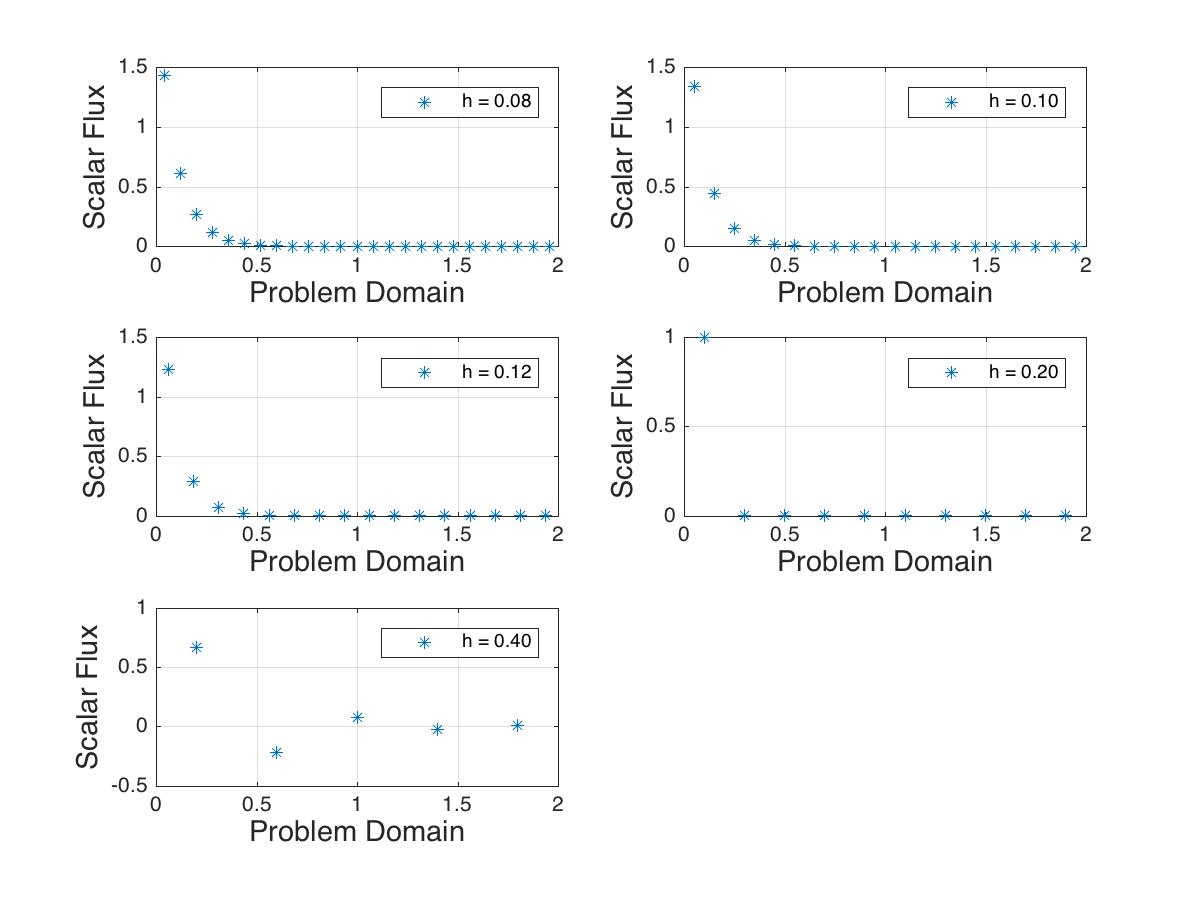
\includegraphics[width=16cm]{ScalarFlux.jpg} % versioned
  \caption{Cell-centered scalar flux for \(h=0.08, 0.1, 0.125, 0.2, 0.4\) and \(\alpha=0\).}
  \label{fig:20}
\end{figure}

As can be seen, negative fluxes are obtained for \(h=0.4\), the largest of the mesh spacings. From Eq. \eqref{eq:NegativeCondition}, the flux can be negative for:

\begin{equation}
\Delta_i>0.2
\end{equation}

The only mesh spacing with \(\Delta_i>0.2\) is the last spacing, of \(h=0.4\). Because negative flux is observed, this shows that the predictions from question 2 are accurate in terms of the needed mesh refinement to avoid the unphysical negative flux that can result.\newline

\textbf{(b)}: Using the same property data, part (a) is repeated for \(\alpha=-0.9, -0.5, 0.25, 0.5, 0.9\). 

\begin{figure}[H]
  \centering
  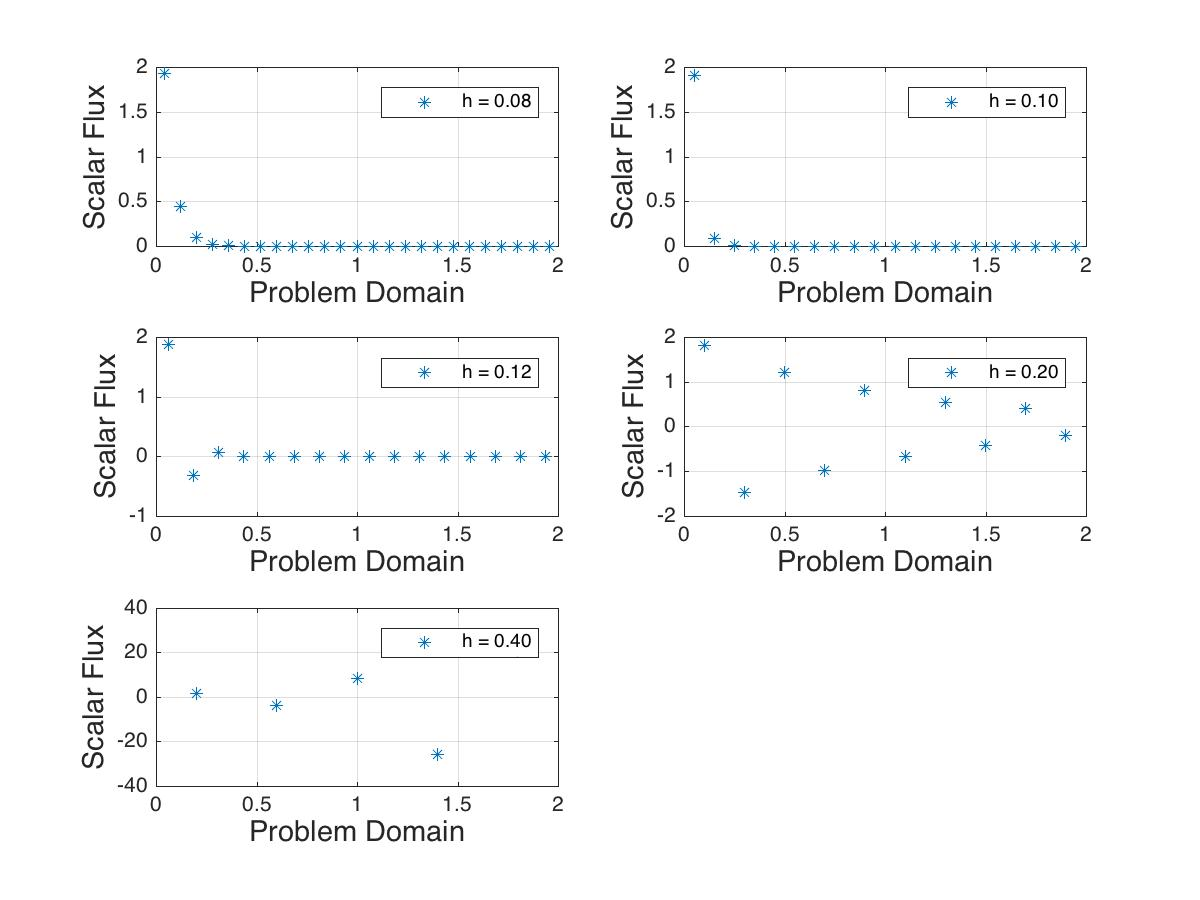
\includegraphics[width=16cm]{ScalarFlux1-90.jpg} % versioned
  \caption{Cell-centered scalar flux for \(h=0.08, 0.1, 0.125, 0.2, 0.4\) and \(\alpha=-0.9\).}
\end{figure}

\begin{figure}[H]
  \centering
  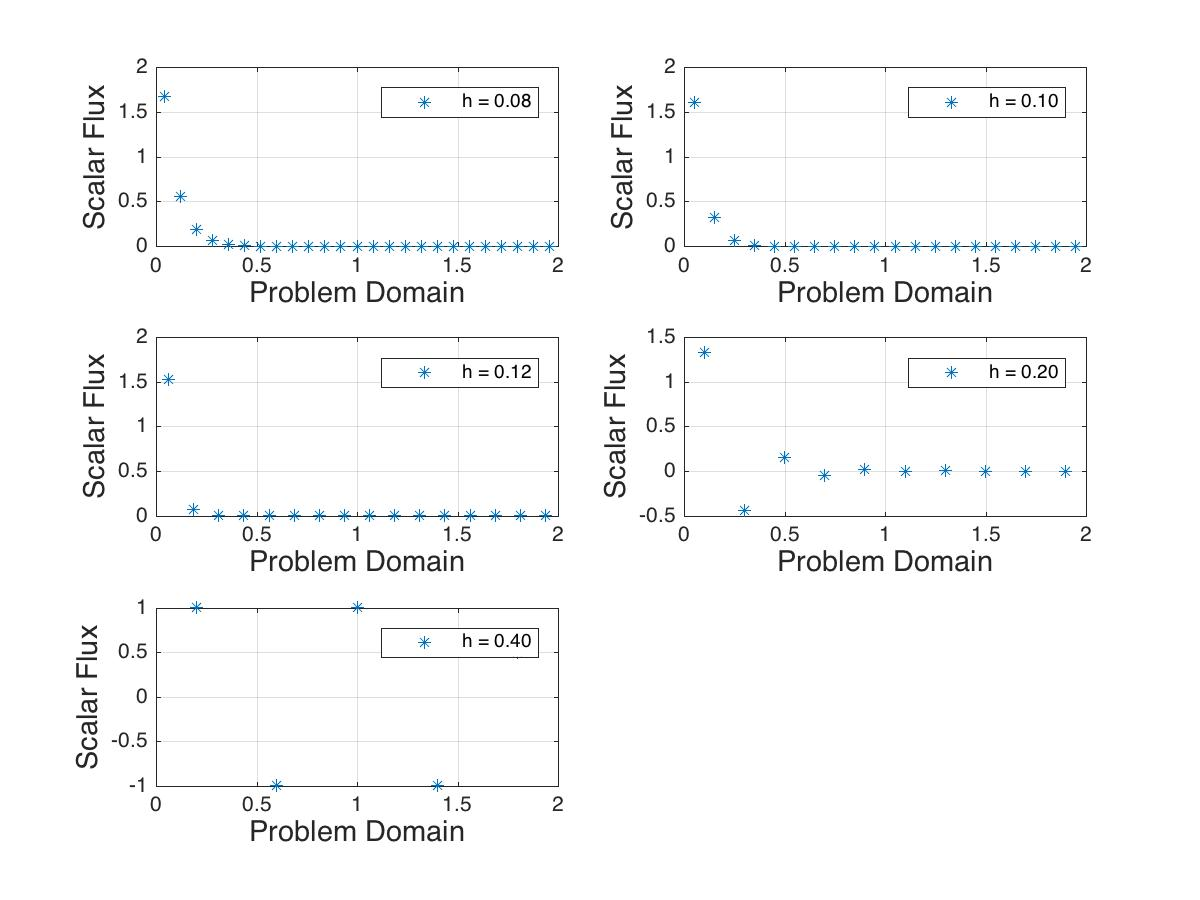
\includegraphics[width=16cm]{ScalarFlux1-50.jpg} % versioned
  \caption{Cell-centered scalar flux for \(h=0.08, 0.1, 0.125, 0.2, 0.4\) and \(\alpha=-0.5\).}
\end{figure}

\begin{figure}[H]
  \centering
  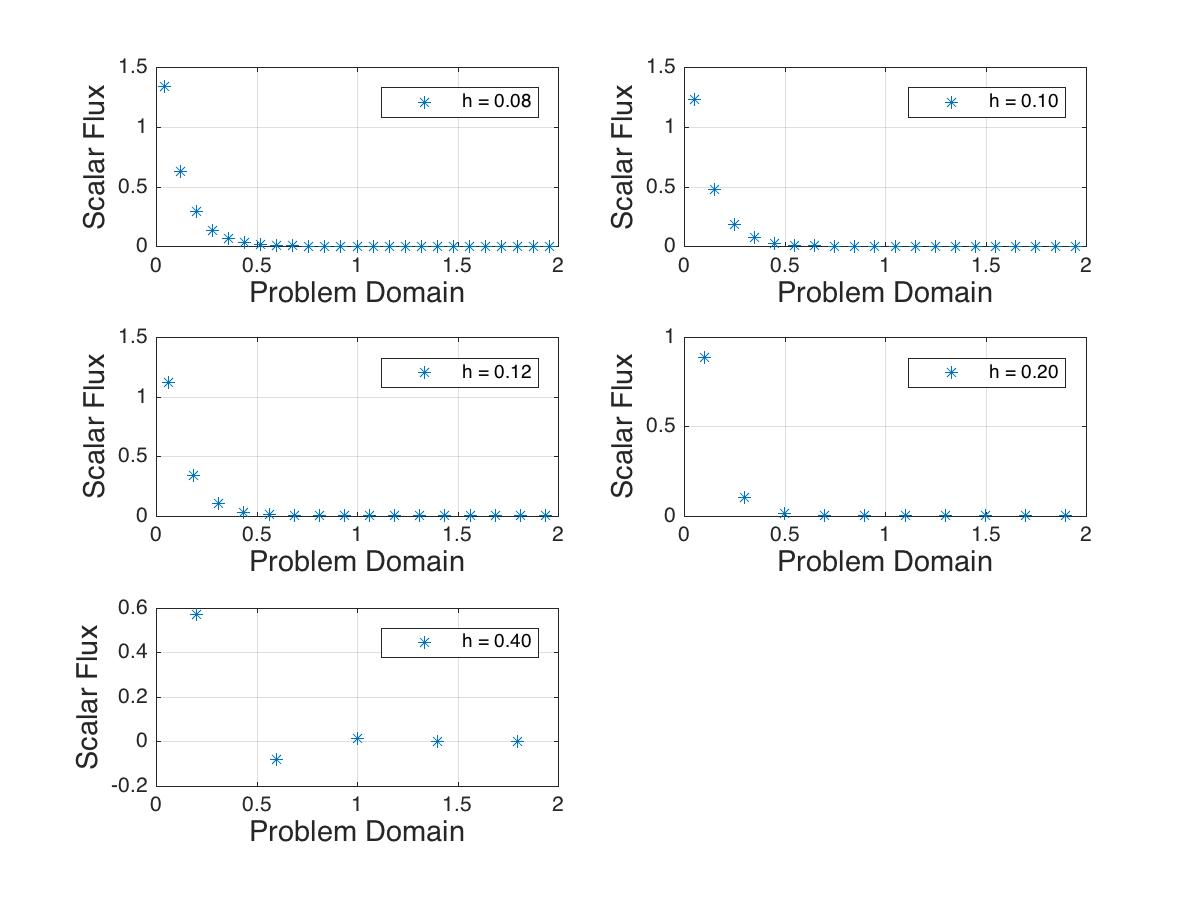
\includegraphics[width=16cm]{ScalarFlux225.jpg} % versioned
  \caption{Cell-centered scalar flux for \(h=0.08, 0.1, 0.125, 0.2, 0.4\) and \(\alpha=0.25\).}
\end{figure}

\begin{figure}[H]
  \centering
  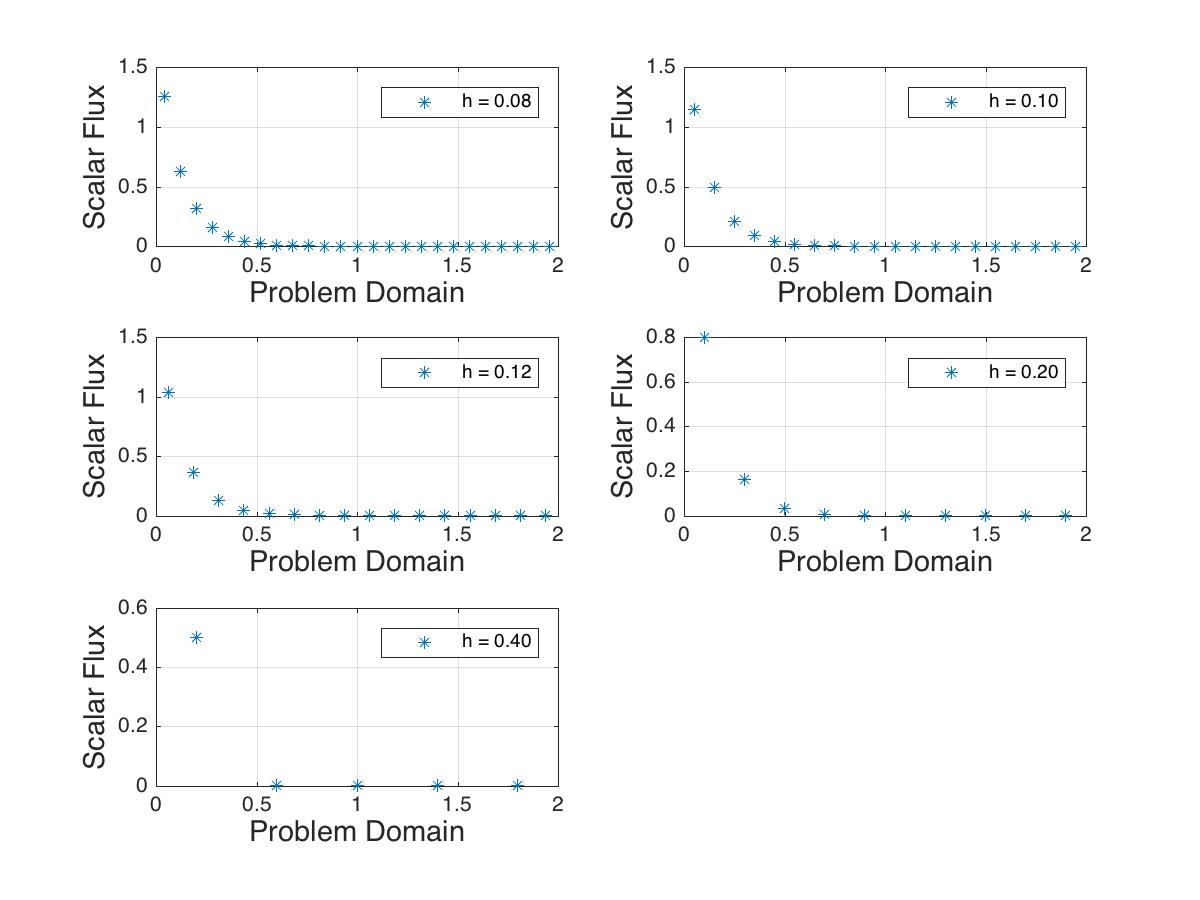
\includegraphics[width=16cm]{ScalarFlux250.jpg} % versioned
  \caption{Cell-centered scalar flux for \(h=0.08, 0.1, 0.125, 0.2, 0.4\) and \(\alpha=0.5\).}
\end{figure}

\begin{figure}[H]
  \centering
  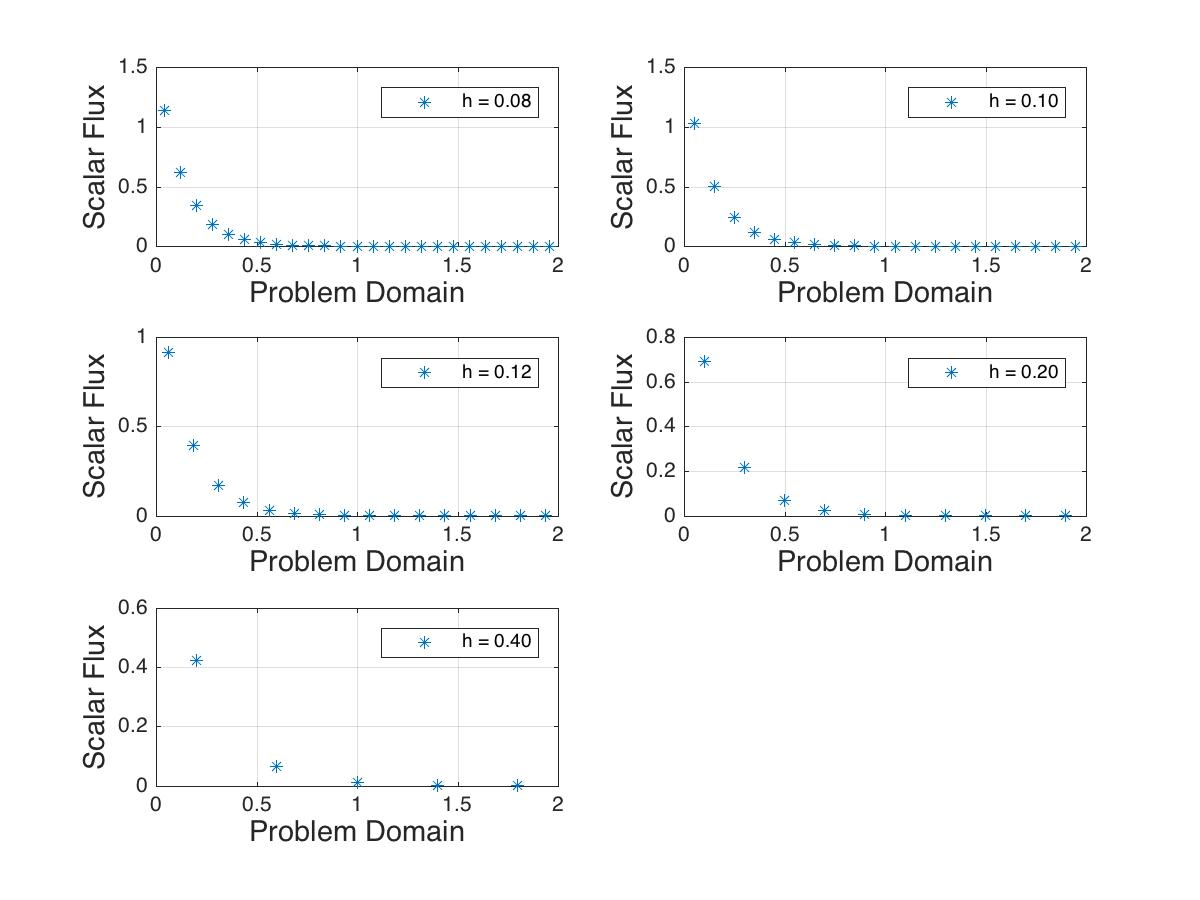
\includegraphics[width=16cm]{ScalarFlux290.jpg} % versioned
  \caption{Cell-centered scalar flux for \(h=0.08, 0.1, 0.125, 0.2, 0.4\) and \(\alpha=0.9\).}
\end{figure}

The impact of changing \(\alpha\) on the accuracy of the solution can be judged by comparing the results with those obtained for \(h=0.08\) and \(\alpha=0\) in Fig. \ref{fig:20} (assuming that such a fine mesh gives the correct answer). The table below summarizes the impact of changing \(\alpha\) on whether or not negative fluxes are obtained or if the solution is unphysical (for example, has oscillations, since that would not be expected to occur for a problem with no complicated source profile). From the figures, it is clear that the less positive the \(\alpha\), the more probable the occurrence of negative flux, oscillations between positive and negative flux, and an inability to capture the smooth exponential decay of the flux beginning at \(x=0\). For instance, while both \(\alpha=0.5\) and \(\alpha=0.9\) give reasonably good results, for \(h=0.4\), \(\alpha=0.5\) fails to capture the smooth decay in flux to zero, and after only one cell sets the flux to zero. On the other hand, for \(\alpha=0.9\), the flux decays with an exponential profile as expected. Hence, \(\alpha=0.9\) should be selected when using this code, at least for the specific case here with no source - it is possible that changing conditions would make the other choices of \(\alpha\) better-suited.

\begin{table}[H]
\caption{Impact on changing \(\alpha\) for the solution in terms of negative flux and physical reality. Solutions that appear to display the correct behavior are indicated as ``good.''}
\centering
\begin{tabular}{c c c c c c}
\hline\hline
\(h\) & \(\alpha=-0.9\) & \(\alpha=-0.5\) & \(\alpha=0.25\) & \(\alpha=0.5\) & \(\alpha=0.9\)\\ [0.5ex]
\hline
0.080 & \textbf{good}			& \textbf{good}		& \textbf{good}		& \textbf{good}			& \textbf{good}\\
0.100 & too-sharp drop-off		& \textbf{good}		& \textbf{good}		& \textbf{good} 			& \textbf{good}\\
0.125 & negative \(\phi\)		& too-sharp drop-off	& \textbf{good}		& \textbf{good} 			& \textbf{good}\\
0.200 & negative \(\phi\)		& negative \(\phi\)	& \textbf{good}		& \textbf{good} 			& \textbf{good}\\
0.400 & negative \(\phi\)		& oscillations		& negative \(\phi\)	& too-sharp drop-off		& \textbf{good}\\
\hline
\end{tabular}
\label{table:3}
\end{table}

\circled{4} The 1-D form of the multigroup transport equation is:

\begin{equation}
\frac{\mu_a}{h_i}\left(\psi_{a,i+1/2}^g-\psi_{a,i-1/2}^g\right)+\Sigma_{t,i}^g\psi_{a,i}^g=2\pi\sum_{a=1}^{N}w_a\underbrace{\sum_{g^{'}=1}^G\Sigma_{s,i}(g^{'}\rightarrow g, a^{'}\rightarrow a)\psi_{a^{'},i}^{g^{'}}}_\text{in-scattering}+\underbrace{\frac{\chi_g}{2}\sum_{g^{'}=1}^{G}\nu_{g^{'}}\Sigma_{f,i}^{g^{'}}\phi_{i}^{g^{'}}}_\text{fission}+\frac{1}{2}Q_i^g\\
\end{equation}

Writing the general system of equations for five groups (\(G=5\)) (each equation applies to a single angular direction \(\mu_a\)) gives:

\begin{equation}
\begin{aligned}
\frac{\mu_a}{h_i}\left(\psi_{a,i+1/2}^1-\psi_{a,i-1/2}^1\right)+\Sigma_{t,i}^1\psi_{a,i}^1=2\pi\sum_{a=1}^{N}w_a\sum_{g^{'}=1}^2\Sigma_{s,i}(g^{'}\rightarrow 1, a^{'}\rightarrow a)\psi_{a^{'},i}^{g^{'}}+\frac{\chi_1}{2}\sum_{g^{'}=1}^{G}\nu_{g^{'}}\Sigma_{f,i}^{g^{'}}\phi_{i}^{g^{'}}+\frac{1}{2}Q_i^1\\
\frac{\mu_a}{h_i}\left(\psi_{a,i+1/2}^2-\psi_{a,i-1/2}^2\right)+\Sigma_{t,i}^2\psi_{a,i}^2=2\pi\sum_{a=1}^{N}w_a\sum_{g^{'}=1}^2\Sigma_{s,i}(g^{'}\rightarrow 2, a^{'}\rightarrow a)\psi_{a^{'},i}^{g^{'}}+\frac{\chi_2}{2}\sum_{g^{'}=1}^{G}\nu_{g^{'}}\Sigma_{f,i}^{g^{'}}\phi_{i}^{g^{'}}+\frac{1}{2}Q_i^2\\
\frac{\mu_a}{h_i}\left(\psi_{a,i+1/2}^3-\psi_{a,i-1/2}^3\right)+\Sigma_{t,i}^3\psi_{a,i}^3=2\pi\sum_{a=1}^{N}w_a\sum_{g^{'}=1}^5\Sigma_{s,i}(g^{'}\rightarrow 3, a^{'}\rightarrow a)\psi_{a^{'},i}^{g^{'}}+\frac{\chi_3}{2}\sum_{g^{'}=1}^{G}\nu_{g^{'}}\Sigma_{f,i}^{g^{'}}\phi_{i}^{g^{'}}+\frac{1}{2}Q_i^3\\
\frac{\mu_a}{h_i}\left(\psi_{a,i+1/2}^4-\psi_{a,i-1/2}^4\right)+\Sigma_{t,i}^4\psi_{a,i}^4=2\pi\sum_{a=1}^{N}w_a\sum_{g^{'}=1}^5\Sigma_{s,i}(g^{'}\rightarrow 4, a^{'}\rightarrow a)\psi_{a^{'},i}^{g^{'}}+\frac{\chi_4}{2}\sum_{g^{'}=1}^{G}\nu_{g^{'}}\Sigma_{f,i}^{g^{'}}\phi_{i}^{g^{'}}+\frac{1}{2}Q_i^4\\
\frac{\mu_a}{h_i}\left(\psi_{a,i+1/2}^5-\psi_{a,i-1/2}^5\right)+\Sigma_{t,i}^5\psi_{a,i}^5=2\pi\sum_{a=1}^{N}w_a\sum_{g^{'}=1}^5\Sigma_{s,i}(g^{'}\rightarrow 5, a^{'}\rightarrow a)\psi_{a^{'},i}^{g^{'}}+\frac{\chi_5}{2}\sum_{g^{'}=1}^{G}\nu_{g^{'}}\Sigma_{f,i}^{g^{'}}\phi_{i}^{g^{'}}+\frac{1}{2}Q_i^5\\
\end{aligned}
\end{equation}

Because neutrons are assumed to not be able to scatter from thermal groups to fast groups, \(\Sigma_{s,i}(3,4,5\rightarrow 1,2\) is zero, where the numbers listed as comma-separated values are intended to indicate that, for example, \(\Sigma_{s,i}(3\rightarrow 1)=0\), \(\Sigma_{s,i}(3\rightarrow 2)=0\), \(\cdots\) , and \(\Sigma_{s,i}(5\rightarrow2)=0\). It is assumed that neutrons of any energy levels can induce fission, and the external source contributes neutrons of all energies. Also, while it is typical to assume that no thermal neutrons are born from fission (\(\chi_3=\chi_4=\chi_5=0\)), this is not assumed here based on the problem statement.

Because the thermal groups are assumed to upscatter, for groups 3, 4, and 5, neutrons of any group can scatter into groups 3, 4, and 5.

\section{Appendix}
This section contains all the code used for each question. 

%\subsection{Question 2}
%\lstinputlisting[language=Matlab]{Q2.m}


\end{document}